\documentclass{article}

\usepackage{amsmath}
\usepackage{graphicx}

\begin{document}

The hash function is defined by initially choosing $M = \lceil 2(sm^2)\log(sm^2)
\rceil$ and choosing a random prime $p$ in the range $1,...,M$, and then returning
the input mod $p$.

Matrix $M$ of size $(n - m + 1)^2$ represents the values of the $m \times m$
contiguous submatrices at all positions in $T$ interpreted as $m^2$-bit
integers.

If we assume the first row and column of $M$ are calculated, the rest can be
computed using this recurrence:

$$M[i,j] = x[i+m-1, j+m-1] +$$
$$2M[i - j - 1] + 2^mM[i - 1, j] + 2^{m+1}M[i-1,j-1]$$
$$+2^{m^2+m}x[i-1, j-1] - 2^mx[i+m-1,j+1]-2^{m^2}x[i-1,j-m+1]$$

Intuitively, the bits in the two submatrices immediately up and to the left
are being shifted to the positions relative to the new submatrix, and the
submatrix diagonally up and to the left one unit is being shifted in the same
way and subtracted off to cancel overlapping terms and most of the old terms
from those two submatrices. Finally, the 4 corner values have to be manually
corrected.

\begin{figure}[h!]
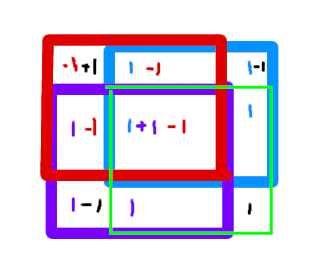
\includegraphics[scale=3]{diagram}
    \caption{Green is M[i,j], blue is M[i,j-1], purple is M[i-1,j], and red is
    M[i-1,j-1]. The other terms are represented in black.}
\end{figure}


$$M[i,j] \mod p = (x[i+m-1, j+m-1] \mod p +$$
$$2M[i - j - 1] \mod p + 2^mM[i - 1, j] \mod p+ 2^{m+1}M[i-1,j-1] \mod p$$
$$+2^{m^2+m}x[i-1, j-1] \mod p - 2^mx[i+m-1,j+1] \mod
p-2^{m^2}x[i-1,j-m+1]\mod p) \mod p$$

$$M[i,j] \mod p = (x[i+m-1, j+m-1] +$$
$$2(M[i - j - 1] \mod p) + (2^m \mod p) (M[i - 1, j] \mod p)+ (2^{m+1} \mod
p)(M[i-1,j-1] \mod p)$$
$$+(2^{m^2+m} \mod p)x[i-1, j-1] - (2^m \mod p)x[i+m-1,j+1] - (2^{m^2} \mod p)x[i-1,j-m+1]) \mod p$$

$$h(M[i,j]) = (x[i+m-1, j+m-1] +$$
$$2h(M[i - j - 1]) + h(2^m) h(M[i - 1, j]) + h(2^{m+1})h(M[i-1,j-1])$$
$$+h(2^{m^2+m})x[i-1, j-1] - h(2^m)x[i+m-1,j+1] - h(2^{m^2})x[i-1,j-m+1]) \mod p$$

So instead of storing $M$, we store a matrix $H$ such that $H[i,j] =
h(M[i,j])$.

The values $h(2^m)$, $h(2^m+1)$, $h(2^{m^2+m})$, and $h(2^{m^2})$ can be
pre-computed.

We compute $H[0,0]$ first through brute force in $O(m^2)$ time. then, we
compute the first row and column of $H$ with a similar rolling hash idea in
$O(m)$ time. Finally, we can compute the remaining entries in constant time
by first computing the second column starting from the top, then the third,
and so on.

At any point, if the hash value matches the pre-computed hash value of $P$, we
have found a (probable) match, so return the current index.

The rolling hash computation for the first row and column of $H$ is to
subtract the bit-shifted values of the entire old row or column that is not shared by the new
window and adding the bit-shifted values of the new row or column in the hash
computation. This should be an $O(m)$ operation.

Running time analysis:

pre-computing the constant hash values requires $O(m^2)$ time. Computing the
0,0 entry by brute force takes $O(m^2)$ time. Computing the first row and
column takes $O(nm)$ time. Computing the rest of the entries takes
$O(n^2)$ time. Thus, the algorithm runs in overall $O(n^2)$ time.

Error analysis:

For some $m \times m$ submatrix $S$ of $T$, if its hash does not match the hash of $P$,
there is no way that $S = P$.

If it does match, but $S \neq P$, the probability of that happening is the
same as the probability of a hash collision for distinct elements, or $1/s$,
where $M = \lceil 2(sm^2)\log(sm^2) \rceil$ is the $M$ used in the hash function.

By the union bound, the probability of a collision happening in any of the
submatrices is less than $n^2/s$.

\pagebreak

First, compute the hash values of each of the rows of $P$.

\end{document}
